\newpage

\chapter{Electronics Design}

Electronics section overview ...

\newpage

\section{Raspberry Pi setup}

Pi voltage range = 1.8V to 3.3V (High)

\newpage

\section{Speed Sensor Design}

Speed sensors are required to measure the rotational speed of the two rear drums. For the application, RPR-220 infrared photoreflectors were used as they allow for reliable contactless speed measurements. The RPR-220 unit was also readily available, inexpensive and would work with the Raspberry Pi's \acs{gpio} pins.

\begin{table}[H]
		\renewcommand{\arraystretch}{\tablestretch}
	\centering
	\caption{RPR-220 Data Sheet Parameter Summary}
	\citep{RPR:2015}
	\begin{tabularx}{\textwidth}{X >{\raggedright}p{3cm} >{\raggedright\arraybackslash}p{2cm} }
		\toprule
		Parameter                       & Condition & Value                   \\
		\midrule
		LED Current                     & Maximum   & \SI{50}{\milli\ampere}  \\
		LED Voltage                     & Rated     & \SI{5}{\volt}           \\
		Phototransistor Current (Dark)  & Rated     & \SI{0.5}{\micro\ampere} \\
		Phototransistor Current (Light) & Rated     & \SI{0.8}{\milli\ampere} \\
		Phototransistor Current         & Maximum   & \SI{}{\milli\ampere}    \\
		Phototransistor Response Time   & Rated     & \SI{10}{\micro\second}  \\
		\bottomrule
	\end{tabularx}
	\label{tab:rprdata}
\end{table}

The Raspberry Pi is capable of measuring inputs using the standard Rpi.GPIO library up to \SI{5}{\kilo\hertz}. Since the maximum expected drum rotation speed is 3500 \acs{rpm}, which equates to \SI{66.6}{\hertz}, the sensors would be capable of handling up to 75 segments per revolution. Considering a safety factor and in order to reduce the data burden, a sensor system implementing 60 segments was selected to ensure high enough resolution at low speeds.

The LED circuit limits the current to \SI{42}{\milli\ampere} with a \SI{120}{\ohm} resistor. The circuit is powered through the CKCY Buck03 \SI{5}{\volt} buck converter. The \acs{led} is powered by an external power source to avoid damaging Raspberry Pi's \acs{gpio} pins, and to allow for it to operate at \SI{5}{\volt}. The phototransistor lets \SI{0.8}{\milli\ampere} pass if \SI{100}{\percent} of the transmitted light is reflected. A voltage divider circuit was used to achieve a \SI{3.3}{\volt} reading on the output to the Raspberry Pi \ac{gpio} pin, where the resistance value was determined with equation \ref{eq:ohm}. 

\begin{equation}
	R = \frac{V}{I}
	\label{eq:ohm}
\end{equation}

\begin{figure}[H]
	\centering
	\begin{subfigure}[t]{.315\textwidth}
		\centering
		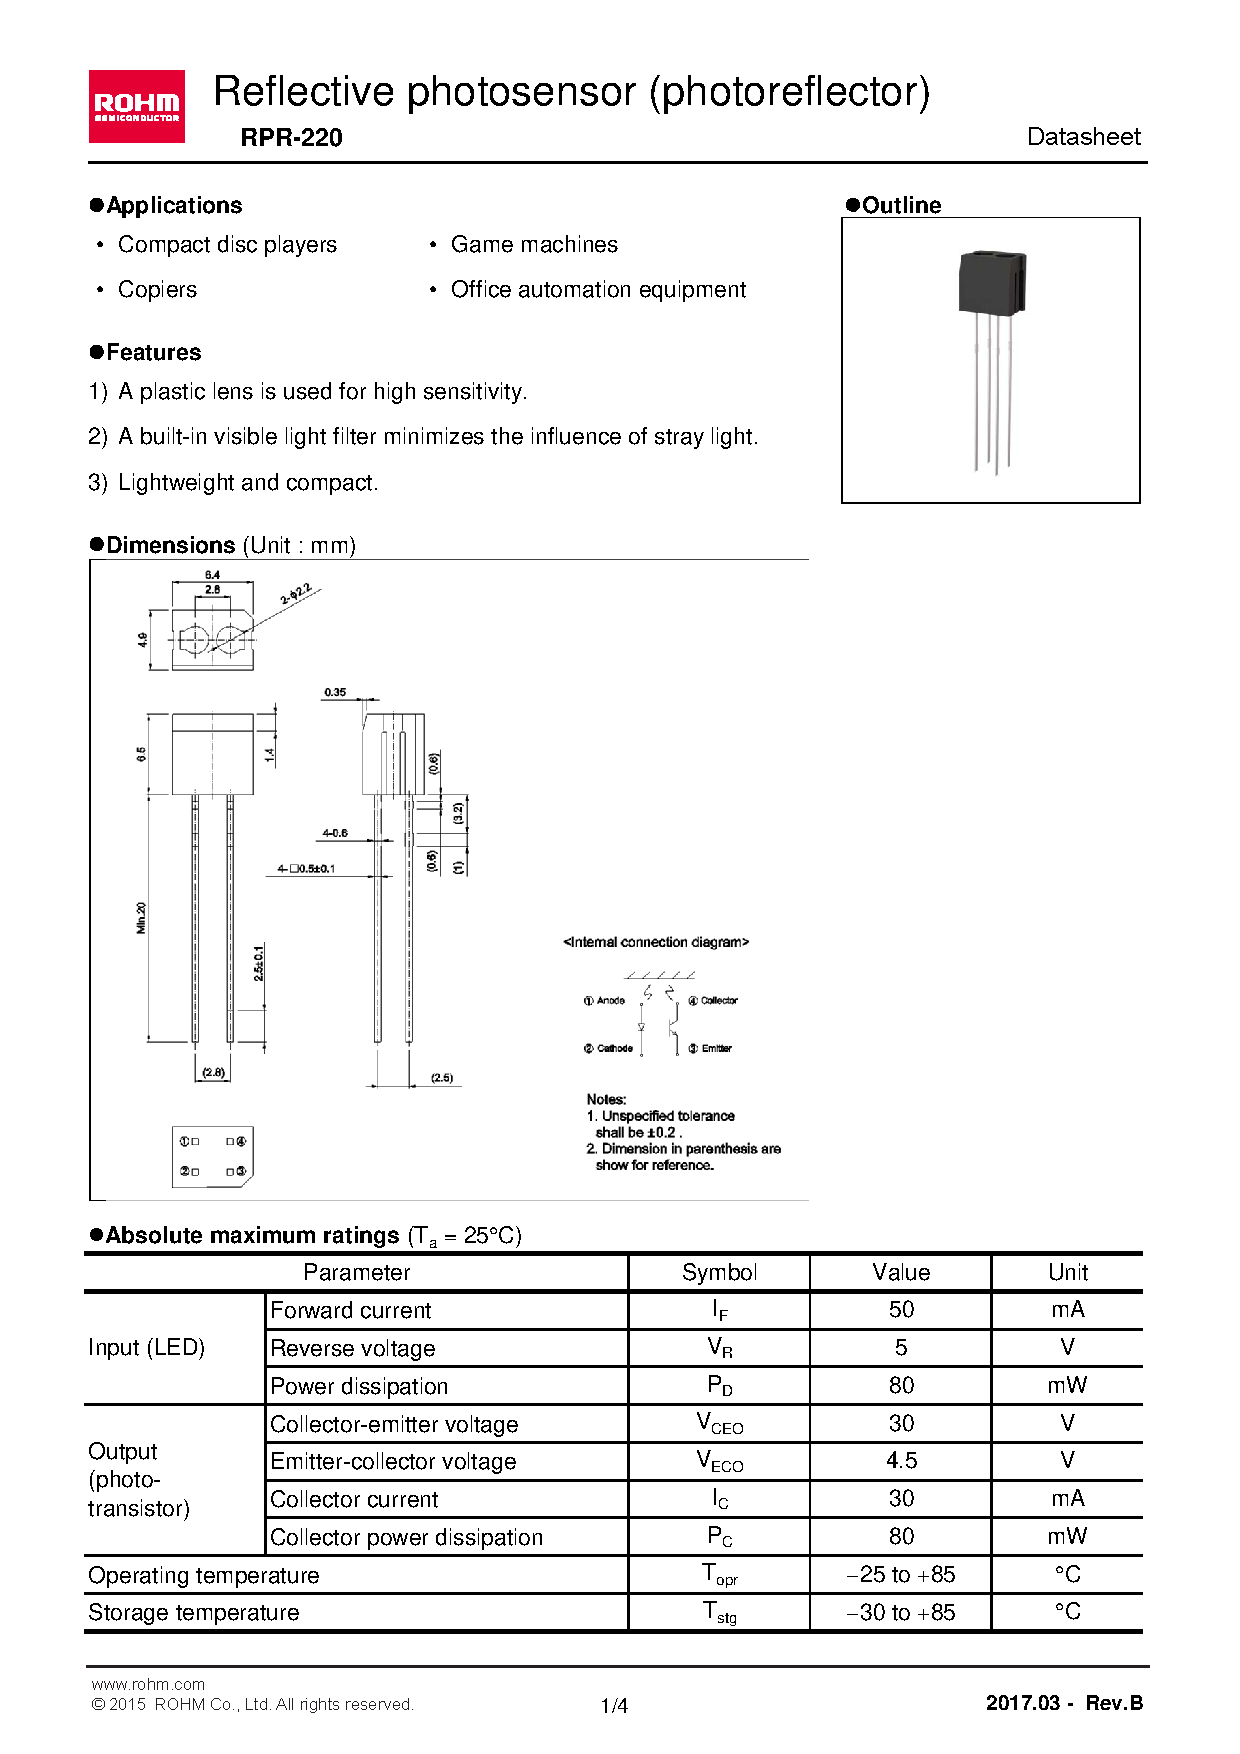
\includegraphics[width = \linewidth]{RPR220.jpg}
		\caption{RPR-220 Photoreflector}
		\citep{RPR:2015}
		\label{fig:rpr}
	\end{subfigure}
	\begin{subfigure}[t]{.65\textwidth}
		\centering
		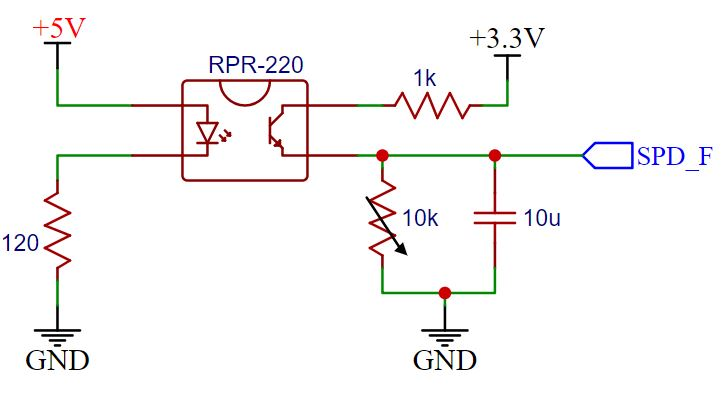
\includegraphics[width = \linewidth]{SensorCircuit.JPG}
		\caption{Sensor Biasing and Filter Circuit}
		\label{fig:sensorD}
	\end{subfigure}
	\caption{Sensor Design}
	\label{fig:Sensor}
\end{figure}

Thus, with the \SI{3.3}{\volt} source and \SI{0.8}{\milli\ampere} of current, the resistor value can be calculated using equation \ref{eq:ohm} as \SI{4125}{\ohm}. This, however, is for the ideal case, and a much lower percentage can be expected to reflect when the sensor is implemented. For the design, a reflection of \SI{90}{\percent} at a distance of \SI{6}{\milli\meter} where the data sheet indicates the current will be \SI{0.3}{\milli\ampere}. Following the same calculation, a resistor value of \SI{11}{\kilo\ohm} is determined.

\begin{equation}
	f_c = \frac{1}{2 R C}
\end{equation}

\newpage

\section{Motor Control}

For controlling the phase of the magnets of the Eddy Current brake, a stepper motor was chosen for it's accuracy and the ability to control it's operation with the Raspberry Pi's \acs{gpio} pins.

\begin{figure}[H]
	\centering
	\begin{subfigure}[t]{.550\textwidth}
		\centering
		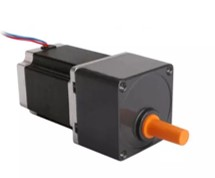
\includegraphics[height = 3cm]{StepperMotor.jpg}
		\caption{Nema 23 Stepper Motor with 15:1 Gearbox}
		\citep{Robotics:2022}
		\label{fig:stepper}
	\end{subfigure}
	\begin{subfigure}[t]{.41\textwidth}
		\centering
		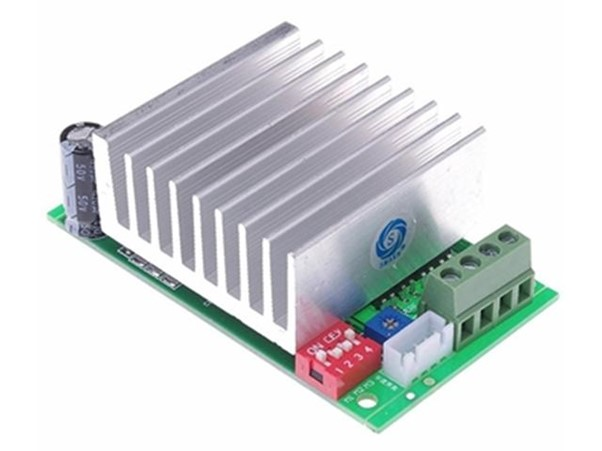
\includegraphics[height = 2.5cm]{StepperDriver.jpg}
		\caption{TB660 v1.1 Stepper Motor Driver}
		\citep{Communica:2022}
		\label{fig:motorDriver}
	\end{subfigure}
	\caption{Motor Control Components}
	\label{fig:Motor}
\end{figure}



After testing the resistance level between the wires on the Nema-23 stepper motor, the results were:

\begin{table}[H]
		\renewcommand{\arraystretch}{\tablestretch}
	\centering
	\caption{Stepper Motor Wire Resistance Measurement Results}
	\begin{tabularx}{\textwidth}{X X X X X X  }
		\toprule
		       & Black               & Green                 & Red                   & Yellow                & White                 \\
		\midrule
		Blue   & > \SI{1}{\mega\ohm} & > \SI{1}{\mega\ohm}   & \SI{41.2}{\ohm}       & > \SI{1}{\mega\ohm}   & \SI{20.7}{\ohm}       \\
		White  & > \SI{1}{\mega\ohm} & > \SI{1}{\mega\ohm}   & \SI{20.8}{\ohm}       & > \SI{1}{\mega\ohm}   & \cellcolor{lightgray} \\
		Yellow & \SI{20.7}{\ohm}     & \SI{20.5}{\ohm}       & > \SI{1}{\mega\ohm}   & \cellcolor{lightgray} & \cellcolor{lightgray} \\
		Red    & > \SI{1}{\mega\ohm} & > \SI{1}{\mega\ohm}   & \cellcolor{lightgray} & \cellcolor{lightgray} & \cellcolor{lightgray} \\
		Green  & \SI{40.5}{\ohm}     & \cellcolor{lightgray} & \cellcolor{lightgray} & \cellcolor{lightgray} & \cellcolor{lightgray} \\
		\bottomrule
	\end{tabularx}
	\label{tab:nemaTest}
\end{table}

From Table \ref{tab:nemaTest} above, the wires associated with each coil can be identified. A resistance of > \SI{1}{\mega\ohm} indicates that the wires are not connected to the same coil. For the wires on the same coil, a larger resistance indicates that there is more coiled wire between the connections, and they are thus farther apart. This results in the :

\begin{figure}[H]
	\begin{center}
		
\includegraphics[width=0.3\textwidth]{MotorWire.jpg}
		\caption{Nema-23 Wiring}
		\label{fig:motorWire}
	\end{center}
\end{figure}

\section{Electronics Overview}
